%%%%%%%%%%%%%%%%%%%%%%%%%%%%%%%%%%%%%%%%%%%%%%%%%%%%%%%%%%%%%%%%%%%%%%
% Template Source: Dave Richeson (divisbyzero.com), Dickinson College
% Author: Louis Dod (13bytes.de)
%%%%%%%%%%%%%%%%%%%%%%%%%%%%%%%%%%%%%%%%%%%%%%%%%%%%%%%%%%%%%%%%%%%%%%
% Please report any errors either via pull request, issue (https://github.com/13Bytes/Uni-Merkzettel) or mail (coding@13bytes.de)
% Improvements are also gladly accepted
%%%%%%%%%%%%%%%%%%%%%%%%%%%%%%%%%%%%%%%%%%%%%%%%%%%%%%%%%%%%%%%%%%%%%%


\documentclass[a4paper,10pt,landscape]{article}
\usepackage{fontspec}
\usepackage[T1,EU1]{fontenc}
\usepackage{lmodern}    % font
\usepackage[frenchb]{babel} 
\usepackage{amssymb,amsmath,amsthm,amsfonts}
\usepackage{multicol,multirow}
\usepackage{calc}
\usepackage{ifthen}
\usepackage{mathrsfs}
\usepackage[landscape]{geometry}
\usepackage[colorlinks=true,citecolor=blue,linkcolor=blue]{hyperref}
\usepackage[colorinlistoftodos, ngerman]{todonotes}
\usepackage{xcolor,soul}
\usepackage{cancel}
\usepackage{multirow}
\usepackage{mathabx}
\definecolor{lime}{RGB}{51, 204, 51}
\definecolor{neptune}{RGB}{131,194,188}
\usepackage{physics}

\ifthenelse{\lengthtest { \paperwidth = 11in}}
    { \geometry{top=0.5in,left=.5in,right=.5in,bottom=.5in} }
	{\ifthenelse{ \lengthtest{ \paperwidth = 297mm}}
		{\geometry{top=.5cm,left=1cm,right=1cm,bottom=.5cm} }
		{\geometry{top=.2cm,left=1cm,right=1cm,bottom=.2cm} }
	}
\pagestyle{empty}
\makeatletter
\renewcommand{\section}{\@startsection{section}{1}{0mm}%
                                {-1ex plus -.5ex minus -.2ex}%
                                {0.5ex plus .2ex}%x
                                {\normalfont\large\bfseries}}
\renewcommand{\subsection}{\@startsection{subsection}{2}{0mm}%
                                {-1explus -.5ex minus -.2ex}%
                                {0.5ex plus .2ex}%
                                {\normalfont\normalsize\bfseries}}
\renewcommand{\subsubsection}{\@startsection{subsubsection}{3}{0mm}%
                                {-1ex plus -.5ex minus -.2ex}%
                                {1ex plus .2ex}%
                                {\normalfont\small\bfseries}}
                                
\newcommand{\OK}{\fcolorbox{black}{lime}{\rule{0pt}{1pt}\rule{1pt}{0pt}}}
\newcommand{\YO}{\fcolorbox{black}{blue}{\rule{0pt}{1pt}\rule{1pt}{0pt}}}
\newcommand{\NO}{\fcolorbox{black}{red}{\rule{0pt}{1pt}\rule{1pt}{0pt}}}
\DeclareRobustCommand{\hlcy}[1]{{\sethlcolor{cyan}\hl{#1}}}
\DeclareRobustCommand{\hlgr}[1]{{\sethlcolor{green}\hl{#1}}}
\newcommand{\bbP}{\mathbb{P}}
\newcommand{\bbR}{\mathbb{R}}
\newcommand{\bbE}{\mathbb{E}}
\newcommand{\x}{\underline{x}}
\newcommand{\X}{\underline{X}}
\newcommand{\y}{\underline{y}}
\newcommand{\Y}{\underline{Y}}
\newcommand{\w}{\underline{w}}
\newcommand*{\tensr}[1]{\underline{\underline{#1}}}
\newcommand{\utheta}{\underline{\theta}}
\newcommand{\uphi}{\underline{\phi}}
\newcommand{\umu}{\underline{\mu}}
\newcommand{\dkl}{\textrm{D}_{\textrm{KL}}}
                
\makeatother
\setcounter{secnumdepth}{0}
\setlength{\parindent}{0pt}
\setlength{\parskip}{0pt plus 0.5ex}
% -----------------------------------------------------------------------
\begin{document}

\raggedright
\footnotesize

Deep Learning - Matr.: \hspace{3cm} Name: \hspace{16cm}
{\tiny{\href{https://github.com/13Bytes/Uni-Merkzettel}{\textcolor{gray}{github.com/13Bytes/Uni-Merkzettel}}}}\\

\begin{multicols*}{3}
    \setlength{\premulticols}{1pt}
    \setlength{\postmulticols}{1pt}
    \setlength{\multicolsep}{1pt}
    \setlength{\columnsep}{2pt}
    % -----------------------------------------------------------------------
   
    
\section{Notation}
    discrete: UPPER CASE \hspace{0.7cm} continuous: lower case\\
    $\ln = \textrm{nats}$ \\
    $y$: latent varaible / ground truth (hidden, not measurable)\\
    $x$: observable variable / measurement \\
    $\hat{y}$: output of DNN\\
    $\odot$ element-wise multiplication\\
    Downstream task (DN): the task you actually want to solve (classification, ...)\\

\section{General stuff}
    \textbf{Matrix \& Math basics}\\
    $(cA)^{-1}=c^{-1}A^{-1}$\\
    $\operatorname {det} \left(A^{-1}\right)=(\det A)^{-1}$\\
    $\partial X^{-1} = -X^{-1} (\partial X) X^{-1}$ \hspace{10pt} (mit $XX^{-1} = I$ und $\partial(I)= 0 $)\\
    $\frac{\partial}{\partial x} x^T \mathbf{B}x = x^T (\mathbf{B} + \mathbf{B}^T) $ \\
    $\|\x\|^2= \x^T\x$\\

    $\log_b(P \cdot Q) = \log_b P + \log_b Q $\\
    $\log_b P^n = n \cdot \log_b P \quad$ so $ \quad \frac{1}{2}\log(x^2) = \log(x)$\\
    Hessian matrix $H(\x) = \begin{bmatrix}
                \frac{\partial^2 f}{\partial x_1^2} & ... & \frac{\partial^2 f}{\partial x_1 \partial x_N}\\
                \cdots & \cdots & \cdots \\
                \frac{\partial^2 f}{\partial x_N \partial x_1} & ... & \frac{\partial^2 f}{\partial x_N^2}\\
                \end{bmatrix}$ \\
    ${\displaystyle x_{1,2}={\frac {-b\pm {\sqrt {b^{2}-4ac}}}{2a}}}$\\
    $(\frac{u}{v})' = \frac{u'v - uv'}{v^2}$\\
    $\lim_{x\to0} x\ln(x) = 0$

    \textbf{Moments of vector}\\
    mean: $\underline{\mu} = \bbE(\X) = \int \x p(\x) d\x 
    \stackrel{\textrm{discrete}}{=} \sum \x_iP(\x_i) $ \\
    correlation: $\mathbf{R} = E(\X\X^\intercal) \int \x\x^\intercal p(\x) d\x
    \stackrel{\textrm{discrete}}{=} \sum \x_i\x_i^\intercal P(\x_i) $ \\
    covariance: $\mathbf{C} = E((\X-\umu)(\X-\umu)^\intercal)
    \stackrel{\textrm{discrete}}{=} \mathbf{R}- \umu\umu^\intercal $ \\
    
    \textbf{Jaccard / IoU} (intersection-over-union)\\
    $0\leq J = \frac{|A \cap B|}{|A \cup B|} =  \frac{|A \cap B|}{|A| + |B| - |A \cap B|} \leq 1$ \\
    \textbf{Dice coefficient}\\
    $0\leq D = \frac{2|A \cap B|}{|A| + |B|}$
    
    \textbf{Chain rule of derivative}\\
    $\dv{f(g(\theta))}{\theta} = \dv{f}{g} \dv{g}{\theta}$

    \textbf{Hyperparameters $\eta$}: configuration parameters, not adapted during training. (Gradient descent not applicable)

    \textbf{time-invariant} shifted input signal $\rightarrow$ shifted output signal $x(n-n_0) \rightarrow y(n-n_0)$ (e.g. convolution 1D)\\
    \textbf{shift-invariant} $x(n_1-i_1, n_2-i_2) \rightarrow y(n_1-i_1, n_2-i_2)$ (e.g. convolution 2D)\\
    \textbf{temporal correlation:} loss of meaning if data is scrambled\\

    \textbf{Inductive bias}: Bias that shapes learning in a desired way (e.g. infrastructure enables things).\\
    - dense layer $\rightarrow$ information from all neurons $\rightarrow$ decision making\\
    - convolutional layer $\rightarrow$ learning of local feature\\
    - recurrent layer $\rightarrow$ learning of temporal correlations\\
    
    \textbf{Cross-correlation} (= attention): find known segment in long measurement \\
    \textbf{Autocorrelation} (= self-attention): find self-similarities beween segments of same signal\\
    \textbf{Neural architecture search (NAS)}: automated search for good fitting DNN architecture\\
    \textbf{Causal inference/reasoning} is beyond ML!\\
    \textbf{Epoche}: one whole pass of all training-samples through the NN. (Consists of $N/B$ minibatches) \\
    {\boldmath $\nabla ||\underline{w}||^2$} $ = 2 \underline{w}$\\
    \textbf{Empirical distribution}: $\hat{p}(x,y) = \frac{1}{N}\delta(\x - \x(n), \ \y - \y(n))$ ($\delta$: Dirac-Kernel)


    \hrule
    \section{Probabilities}
    
    \begin{tabular}{p{4cm}|p{4cm}}
        \textbf{PMF} - $P(\cdot)$  & \textbf{PDF} - $p(\cdot)$ \\
       (probability mass function) & (probability density function)\\
        discrete & continuouse \\
         & \\
    \end{tabular}
    \subsection{Uniform distribution}
     PDF: $ p(x)= \left\{\begin{array}{ll} \frac{1}{b-a} & a\leq x \leq b \\
         0 & \textrm{otherwise}
		\end{array}\right.$ \\
    \subsection{Gaussian/normal distribution}
    PDF: $ p(x)=\frac{1}{\sigma\sqrt{2\pi}} e^{-\frac{1}{2\sigma^2}(x-\mu)^2}$ \\
    $\textrm{mit } \underline{x} \sim \mathcal{N}(\mu, \sigma^2) \textrm{ and } |\mathbf{C}| = \det(\mathbf{C})$ 
    \hspace{10pt} \textcolor{gray}{$\det(\sigma^2 \mathbf{I}) = \sigma^{2d}$}\\
    Mean $ E(\underline{x}) = \underline{\mu} = \frac{1}{N} \sum_{n=1}^N x_n $\\
    Covariance $\mathbf{C} = \textrm{E}[(\underline{x}-\underline{\mu})(\underline{x}-\underline{\mu})^T] = \frac{1}{N} \sum_{n=1}^N (\underline{x_n}-\underline{\hat{\mu}})(\underline{x_n}-\underline{\hat{\mu}})^T$\\
    Contour lines: ellipsoids centered at $ \underline{\mu}$. Direction \& size of principal axes given by eigenvectors of $\mathbf{C}$ 
    

    \subsubsection{Standard Gaussian/normal:}
    $ \textrm{PDF: } p(x) = \frac{1}{\sqrt{2\pi}}e^{-\frac{x^2}{2}}$\\
    \begin{multicols*}{2}
    $\textrm{mit } \underline{x} \sim \mathcal{N}(0,1)$\\
    Q-func: $Q(x) = 1- \int_{-\infty}^x p(z) \mathop{dz}$\\
    \columnbreak
    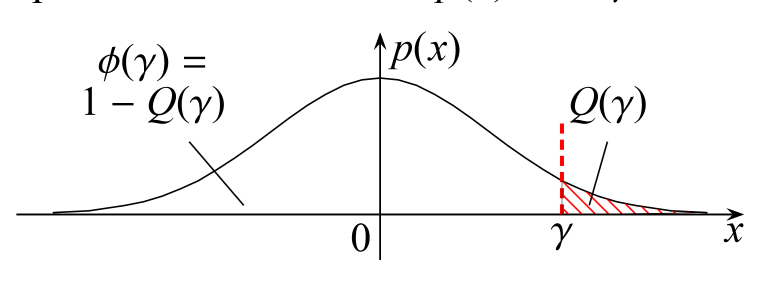
\includegraphics[width=0.10\textwidth]{Graphics/q.png}
    \end{multicols*}
    

    \subsection{Laplace distribution}
    \begin{multicols*}{2}
    $ \textrm{PDF: } p(x) = \frac{1}{2b}\exp\left(\frac{|x-\mu|}{b}\right)$\\
    \columnbreak
    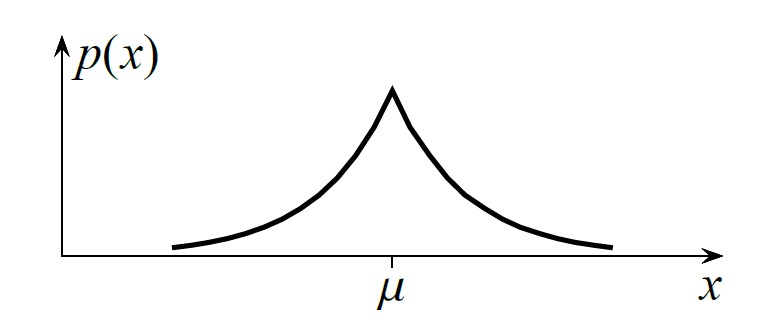
\includegraphics[width=0.10\textwidth]{Graphics/laplace.png} \\
    \end{multicols*}

    \subsection{Bernulli distribution}
    coin-flip
    $X\in\{0,1\}$ \hspace{1cm} $p=P(X=1)>0$ \\
    $ P(x)= \left\{\begin{array}{ll} 1-p & x=0 \\
         p & x=1
		\end{array}\right.$\\


    \hrulefill
    
    \section{Cross Entropy (CE)}
    Entropy $H(X)$: measurement of uncertainty\\
    Between two distributions $X \sim p$ and $Y \sim q(y) $\\
    $H(X,Y) = H(p,q) = -\bbE_{X\sim p}\ln(q(x)) = -\int p(x) \ln(q(x)) dx $

    Applied to \colorbox{yellow}{learning: $H(\hat{p}, q) = \frac{1}{N} \sum_{n=1}^N L(\x(n), \y(n), \underline{\theta} )$}
    
    \section{Kullback-Leibler-Divergence (KLD)}
    Between two distributions $p$ and $q$\\
    $\dkl(p||q) = \int p(x) \ln\left(\frac{p(x)}{q(x)} \right) dx = \bbE_{\x - p(x)}\left[ \ln\left(\frac{p(x)}{q(x)}\right) \right] $\\
    with \textcolor{red}{Gaussian distribution: $\dkl(p\sim \mathcal{N}(\mu_p, \sigma_p^2)||q\sim \mathcal{N}(\mu_q, \sigma_q^2)=\ln(\frac{\sigma_q}{\sigma_p}) + \frac{\sigma_p^2 + (\mu_p - \mu_q)^2}{2 \sigma_q^2} - \frac{1}{2}$ }
    \begin{itemize}
        \item non-negative $\dkl(p||q) \geq 0$
        \item equality $\dkl(p||q) = 0$ if $p(x)=q(x) \forall x$
        \item asymmetry $\dkl(p||q) \neq \dkl(q||p)$ \hspace{0.5cm} forward vs backward ($\rightarrow$ NOT a distance)
        \item additivity  $\dkl(p||q) = \dkl(p_1||q_1) + \dkl(p_2||q_2)$ 
        \\with $x=[x_1, x_2]^\intercal$, all $x_i$ independent ($\rightarrow  p(x) = p(x_1)p(x_2)$)
    \end{itemize}

    \resizebox{\textwidth/3}{!}{
    \begin{tabular}{|c|c|c|}
    \hline
     & \textbf{Forward KL divergence $D_{KL}(p \parallel q)$} & \textbf{Backward KL divergence $D_{KL}(q \parallel p)$} \\
    \hline
    & $p(x) \ln \left(\frac{p(x)}{q(x)}\right)$ & $q(x) \ln \left(\frac{q(x)}{p(x)}\right)$ \\
    $p > q$   & $> 0$ & $ <0$  \\
    $q \to 0$ & \textcolor{red}{$\rightarrow \infty$} &\textcolor{green}{$\rightarrow 0$} \\
    $p \to 0$ & \textcolor{green}{$\rightarrow 0$} & \textcolor{red}{$\rightarrow \infty$} \\
    \hline
    \multicolumn{3}{|c|}{} \\
    \hline
    & Minimize $D_{KL}(p \parallel q)$ & Minimize $D_{KL}(q \parallel p)$ \\
    & $p = 0$: doesn't care about $q$ & $q = 0$: doesn't care about $p$ \\
    & $p > 0$: make $q$ close to $p$ & $q > 0$: make $q$ close to $p$ \\
    \hline
    & ''Zero avoiding'' strategy for $q$: & ''Zero avoiding'' strategy for $q$: \\
    & $q > 0$ if $p > 0$ & $q = 0$ if $p = 0$ \\
    & i.e., makes $q(x)$ \textcolor{green}{broader} than $p(x)$ & i.e., makes $q(x)$ \textcolor{red}{narrower} than $p(x)$ \\
    \hline
    \multicolumn{3}{|c|}{\textbf{Make denominator in $\ln(\cdot)$ broad to minimize $D_{KL}$}} \\
    \hline
    \end{tabular}
}
$\dkl(p||f) = -H(p) + H(p, f) \quad \textrm{as } H(p) \textrm{ fixed}: $\\
$\min_q\dkl(p || q) \hat{=} \min_qH(p || q) \ \Rightarrow  \ \textrm{KLD} 
\hat{=} \textrm{Cross Entropy}$ 

\textbf{Jensen–Shannon divergence}\\
Symetric KLD: $\textrm{D}_{\textrm{JS}} = \frac{1}{2}\left(\dkl\left(p \parallel  \frac{p+q}{2}\right) + \dkl\left(q \parallel \frac{p+q}{2}\right) \right)$

    \hrule
    \section{Neuron}
    $y=\phi(\underline{w}^\intercal \x  +b)$
    
    \hrule
     \section{Initialization}
    \textbf{Zero initialization} is bad! (All neurons behave the same)\\
    Must be Symmetry-breaking!\\
    \textbf{Random initialization} 
    bias: zeros; weight: random \checkmark\\
    e.g. normal or uniform distribution \\
    \textbf{He initialization}\\
    \colorbox{yellow}{Constant activation flow (forward pass)}\\
    through $\textrm{Var}(a_{l,i}) = M_{l-1} \sigma_{w,l}^2\sigma_{x,l-1}^2 $ \\
    $\Rightarrow \sigma_{w,l} \sim \frac{1}{\sqrt{M_{l-1}}}$
    \hspace{5pt} $M_{l-1}$: Fan-in
    
    \textbf{Glorot initialization }\\
    \colorbox{yellow}{Constant gradient flow (forward \& backward pass)}\\
    $||\frac{\partial L}{\partial a}|| = \textrm{const}$ \\
    $\Rightarrow \sigma_{l} \sim \frac{1}{\sqrt{M_{l}}}$
    \hspace{5pt} $M_{l}$: Fan-out

    \section{Hyper-parameter optimization}
    use of a validation-set $D_\textrm{val}$\\
    \textbf{Grid-search:} time-consuming (many params)\\
    \textbf{Bayesian optimization}

    \hrule

    \section{Kernels}
    Create estimate $\hat{p}$ of $p(\x)$ based on samples $\x(n)$\\
    $\hat{p}(\x) = \frac{1}{N}\sum_{n=1}^N k(\x-\x(n))$ with kernel $k(\x)$
    \subsection{Dirac-Kernel}
    $k(\x) = \delta(\x) 
     = \left\{\begin{array}{ll} \infty & x=0 \\
    						  0 & x\neq 0
    	 	\end{array}\right.$
    \hspace{0.3cm} with $\int \delta(x) dx = 1 $
    

    \vfill\null    % ugly fix to achieve formatting
    \columnbreak
    
    \section{Layers}
    weights: $\w \in \mathbb{R}^d $ \\
    bias: $b \in \mathbb{R}$ \\
    activation: $a = \w^\intercal \x + b \in \mathbb{R}$ \\
    activation-function: $\phi: \mathbb{R} \mapsto \mathbb{R}$ \\
    $y = \phi(a)$

    \subsection{> Dense Layer \textcolor{gray}{(ch. 4)}}
    fully connected layer with $c$ neurons \\
    ($c\cdot d$ weights + $c$ bias $\ \Rightarrow c(d+1) $ parameters )
    

    \subsection{> Convolutional layers \textcolor{gray}{(ch. 7)}}
    $A \in \mathbb{R}^{H \times W \times C_\textrm{in}\times C_\textrm{out}}$: height H, width W, channel depth C \\
    \textbf{convolution} wit kernel $h(n)$: $y(n) = \sum_i h(i)x(n-i)$\\
    \textbf{2D convolutional layer} 2D feature map of size $H_l \times W_l$ $\rightarrow$ 3D tensor requires 4D kernel\\
    \textbf{Key ideas:}\\
    \begin{itemize}
        \item Sparse connections: Neuron are only connected to a small subset
        \item Parameter sharing: Params can not be chosen independently. (In CNN: each neuron has the same set pf in- and outgoing weights.
    \end{itemize}
    \textbf{Properties:}\\
    \begin{itemize}
        \item Few parameters (parameter sharing), many multiplications
        \item sparse connections
        \item small receptive field (focus on local patterns)
        \item time-shift invariant (translation-equivariant)
        \item one feature per feature-map
        \item $H_l = H_{l-1}-k_l+1 \ \rightarrow$ image shrinks
    \end{itemize}
    $a_h = \sum_{i=1}^Kw_ix_{h+i-1} \quad 1\leq h \leq H-K+1$\\
    \textbf{Padded convolution:} Zero-padding input to get same output-size as input. $p\geq 0$\\
    \textbf{Strided convolution:} Move kernel by $S\geq 1$ steps (instead of 1) - f.7-9 $\Rightarrow$ Downsampling\\
    \textbf{Dilated convolution:} Let kernel select only every $D \geq 1$'th entry (instead of 1) - f.7-10 $\Rightarrow$ Downsampling\\
    output dimension: $\left\lfloor \frac{H_{l-1}+2P-((K-1)\cdot D+1)}{S} \right\rfloor +1$\\
    Kernel; Padding$=0$; Dilation$=1$; Stride$=1$

     \subsection{> Recurrent layer \textcolor{gray}{(ch. 8)}}
     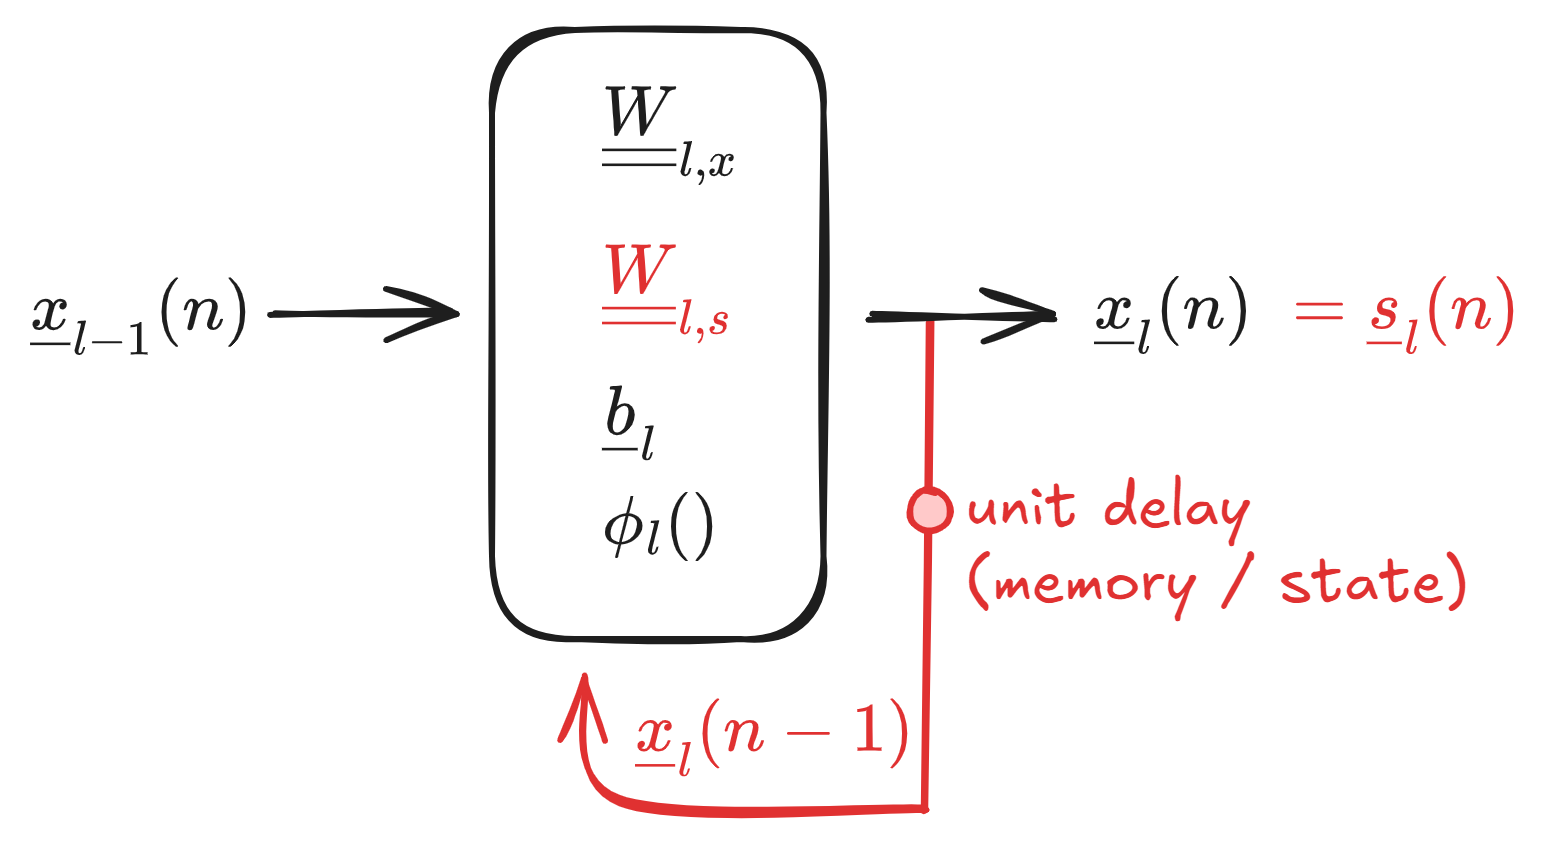
\includegraphics[width=0.6\linewidth]{Graphics/recurrentLayer.png}\\
     \textbf{cross-neuron feedback:} $\tensr{W}_{l,s}$ non-diagonal $\rightarrow$ feedback to also other neurons in this layer
     
     \subsubsection{LSTM layer}
     \begin{multicols*}{2}
        \textbf{Gates} (long short-term memory) :\\
        \begin{itemize}
        \item \textbf{input} (write)
        \item \textbf{forget} (reset)
        \item \textbf{output} (read)
        \end{itemize}
        8 weight matrices \\
    \columnbreak
        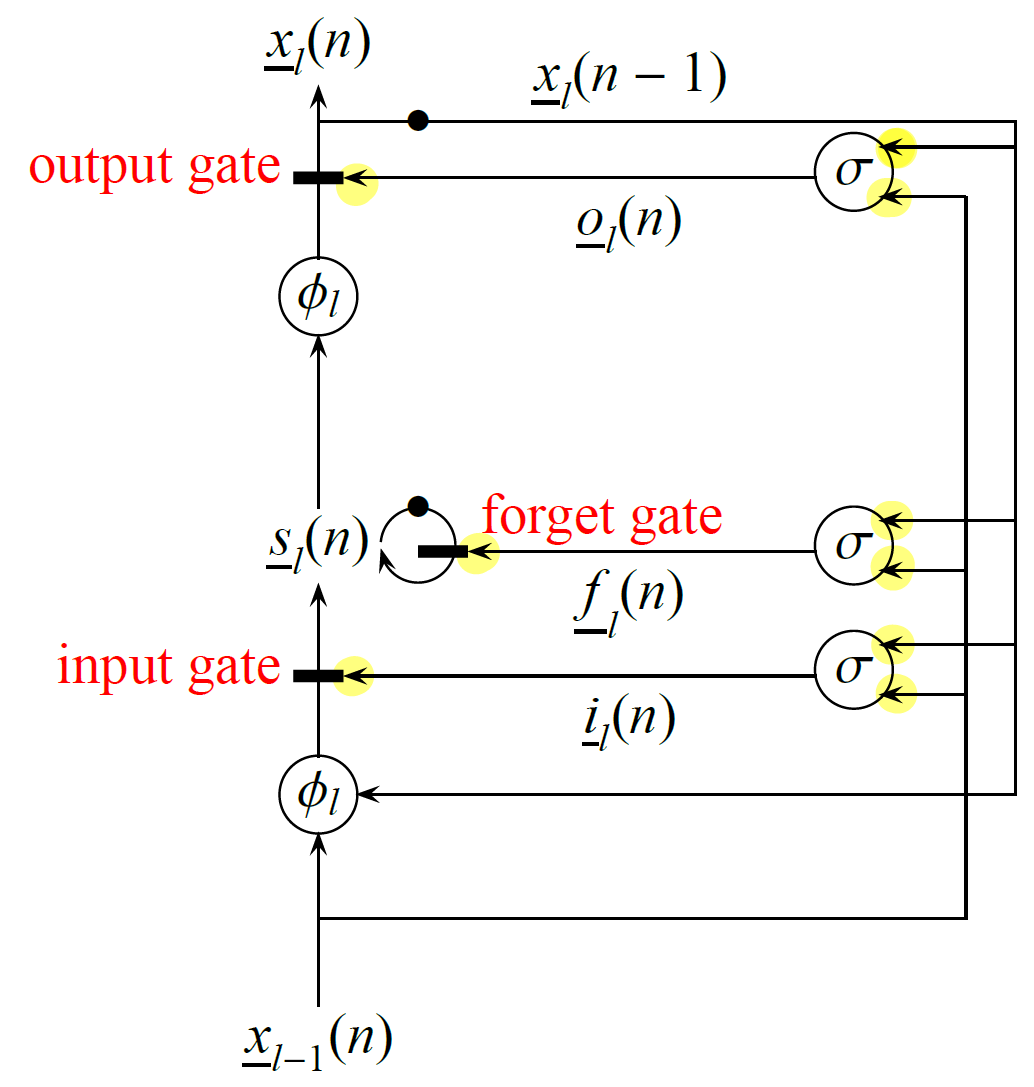
\includegraphics[width=0.8\linewidth]{Graphics/lstm-layer.png}\\
    \end{multicols*}
        $0< \textrm{signal} < 1$\\
        0: close / clear memory \hspace{2pt} - \hspace{2pt}  1: open / keep content\\

    
    \subsection{> Attention \textcolor{gray}{(ch. 9)}}
    \subsubsection{Similarity metric}
   \colorbox{yellow}{\textbf{Scaled dot product:} $\frac{\underline{k}^\intercal \underline{q}}{\sqrt{d}}$ (with dimension $d$)}\\
    \textbf{cosine similarity:} $0\leq \frac{\underline{k}^\intercal \underline{q}}{||\underline{k}||\cdot ||\underline{q}||} \leq 1$\\
    
    \subsubsection{Single-query attention}
    query $q\in \bbR^d$ ($d$ interval dimension)\\
    $N \times$ key-value pairs $k_i, v_i \in \bbR^d $, $\tensr{K}= [k_1, ..,k_N]$, $\tensr{V}$\\
    calc similarities $a_i= s(\underline{q}, \underline{k})$ $\rightarrow$  importance weights $\alpha_i = \textrm{softmax}(a_i)$\\
    $\rightarrow$ refined $v_i$ for $\underline{q}$:  $\textrm{attention}(\underline{q}, \tensr{K}, \tensr{V}) = \sum_{i=0}^N\alpha_i v_i$

    \subsubsection{Multi-query attention}
    multiple queries $\tensr{Q} \in \bbR^{d \times M}$\\
    $\rightarrow M$ attention vectors
    
    \subsubsection{Multi-head attention}
    $h$ heads (each with own dot-product attentions - with own weights from) $\tensr{W}_i^Q, \tensr{W}_i^K, \tensr{W}_i^V$
    
    
    \subsection{Skip connections (Shortcut)}
    over one or multiple layers (identity paths)
    backward pass: $\x_l = \phi_l(W_lx_{l-1}+b_l) + \textcolor{red}{x_{l-1}}$ \\
    $ \frac{\partial \x_l}{\partial \x_{l-1}} = \frac{\partial \phi_l()}{\partial \x_{l-1}} + \textcolor{red}{I}$\\
    Residual connections mandatory for deep networks!
    
    \subsubsection{Normalization}
    (weight normalization ($\tensr{W}$)) and 
    activation normalization  ($\tensr{A}$)\\
    \begin{itemize}
        \item instance normalization (across single channel)
        \item batch normalization (across same channel whole batch)
        \item  layer normalization (across channels)
    \end{itemize}

    
    \subsection{Downsampling layer}
    \textbf{Strided convolution}: \textit{(see ''Convolutional layers'')}\\
    \textbf{Pooling}: 
    max pooling / mean pooling / $l_2$-norm pooling \\
    $\rightarrow$ translation invariance!
    
    \subsection{Upsampling layer}
    \textbf{interpolation}, \textbf{unpooling}, \textbf{deconvolution}
    
    \subsection{Reshaping layer}
     \textbf{flatten layer} $\tensr{X}\in \mathbb{R}^{H\times W \times C} \mapsto  \textrm{vec}(\tensr{X}) \in \mathbb{R}^{H W C}$\\
     \textbf{global average pooling (GAP) layer} reduce each channel/feature to $\mathbb{R}^1$

     \hrule

    

    \section{Activation functions}
    \textbf{linear / identity:}\\
    used in \colorbox{yellow}{output-layer of regression}.\\
    \textbf{Unit step} \\
    $\phi(a) = \left\{\begin{array}{ll} 0 & a<0 \\
						 1 & a>0 \end{array}\right.$
    not differentiable!
    
    \textbf{Sign function} \\
    $\phi(a) = \left\{\begin{array}{ll} -1 & a<0 \\
                     1 & a>0 \end{array}\right. = 2u(a)-1$
    not differentiable!

    \textbf{Sigmoid} \\
    $\phi(a) = \sigma(a) = \frac{1}{1+e^{-a}} $ \\
    $\dv{a}\phi(a) = \phi(a)(1-\phi(a)) $ \\
    \begin{itemize}
        \item $0\leq \phi(a) \leq 1 \ \rightarrow $ good for probabilities 
        \item symmetry
        \item easy computable derivative
    \end{itemize}

    \textbf{Hyperbolic tangent} \\
    $\phi(a) = \tanh(a) = \frac{e^a-e^{-a}}{e^a+e^{-a}}$ \\
    $\dv{a}\phi(a) = 1 - \phi(a)^2 $ \\
    \begin{itemize}
        \item like sigmoid with other output range
    \end{itemize}

    \textbf{ReLU Rectified linear unit} \\
    $\phi(a) = \textrm{Relu}(a) =  \left\{\begin{array}{ll} a & a>0 \\
						 0 & a\leq 0 \end{array}\right. = \max(a,0) $ \\
   $\dv{a}\phi(a) = \left\{\begin{array}{ll} 1 & a>0 \\
						 0 & a< 0 \\
                        1 \textrm{ or } 1 & a=0 \end{array}\right.$ \\
    \begin{itemize}
        \item verry simple
        \item easy derivative
        \item zero-gradient for $a<0 $ (bad)  $\Rightarrow$  \\
        Leaky ReLU $ = \left\{\begin{array}{ll} a & a> 0 \\
						 0.01a & a\leq 0 \end{array}\right.$ \\
    \end{itemize}

    \textbf{Softmax} \\
    $\phi(a): \bbR^c \mapsto \bbR^c$ \\
    $\phi(a) = [\phi_1(a),\ldots, \phi_c(a)]^\intercal$ \hspace{5pt} with \textcolor{red}{$\phi_i(a) = \frac{e^{a_i}}{\sum_{j=1}^ce^{a_j}}$} \\
    $\dv{a_j}\phi_i(a) = \left\{\begin{array}{ll} -\phi_i(a)(1-\phi_i(a)) & i=j \\
						                       -\phi_i(a)\phi_j(a) & i\neq j  \end{array}\right. 
                             = \phi_i(a)(\delta_{ij}-\phi_j(a))$ \\
    \textcolor{gray}{Binary case: $\phi_1(a) = \sigma(a_1-a_2)$ and $\phi_2(a) = 1- \phi_1(a) $} \\
    Used for \colorbox{yellow}{output-layer} (normalization of \colorbox{yellow}{classification-problems})

    
    \vfill\null    % ugly fix to achieve formatting
    \columnbreak

    \section{Loss functions}
    Loss $l(\x,\y, \utheta)$: quality of prediction of one pair \\
    Cost function $L(\utheta)$: average loss over all training samples\\
    $\y=f(\x;\utheta) + \textrm{noise}$ \hspace{10pt} $\y | \x$ Distribution of y given x
    
    \subsection{$L_2$-loss}
    mean square error (MSE) - (white Gaussian noise $\mathcal{N}(0, \sigma^2I)$)\\
    $l(\x,\y;\utheta)= || \y-f(\x; \utheta) ||^2$\\
    $L(\utheta) = \frac{1}{N}\sum_{n=1}^N ||\y(n)-f(\x(n); \utheta)||^2$

    \subsection{$L_1$-loss}
    mean absolute error (MAE) - (Laplace distribution)
    $l(\x,\y;\utheta)= \frac{1}{b} || \y-f(\x; \utheta) ||_1 + \textrm{const} $\\
    $L(\utheta) = \frac{1}{N}\sum_{n=1}^N||\y(n)-f(\x(n); \utheta)||_1$

    \subsection{Categorical CE loss}
    $y\in \{\underline{e}_1, \ldots, \underline{e}_c \}$ (class-labels one-hot coded) \textbf{for classification}\\
    $p$ is approximated by $Q(\y | \y; \utheta) = \prod_{i=0}^c f_i^{y_i}$ \\
    $l(\x,\y;\utheta)= -\ln Q(\y | \y; \utheta) = -y^\intercal \ln(f(\x; \utheta)) $
    (improvement: focal loss $l(\x,\y;\utheta)= -y^\intercal (1-f)^\gamma \odot \ln(f(\x; \utheta)) $)

    \vspace{10pt}
    $\uparrow$ distribution-based loss\\
    $\downarrow$ region-based loss\\
    \vspace{10pt}

    \subsection{IoU and Dice loss}
    IoU: $1-J = 1-\frac{|A \cap B|}{|A| + |B| - |A \cap B|} $\\
    Dice: $1-D = 1- \frac{2|A \cap B|}{|A| + |B|}$ \\
    Independent of region of background. \\
    For multi-class segmentation: $J = \frac{1}{c} \sum_{i=1}^c J_i$

    $|A \cap B| = \sum_h \sum_w \y_{hw} \odot \hat{\y}_{hw} =: \alpha$ \\
    $|A| + |B| = \sum_h \sum_w \y_{hw} + \hat{\y}_{hw} =: \beta$ \\

    Soft IoU and Dice loss: $J = \frac{\alpha \textcolor{red}{+ \epsilon}}{\beta -  \alpha \textcolor{red}{+ \epsilon}}$ $\Rightarrow$ no \textdiv 0\\
    Use Soft for training!
    

    \hrule
    
    \section{Important networks}
    \textbf{MNISTnet3:} 
    CNN for digit recognition on MNIST\\
    \textbf{CIFAR10net:} 
    CNN for image recognition (on CIFAR-10)\\
    \textbf{ResNet:} 
    stack of residual blocks\\
    \textbf{U-Net:} 
    semantic image segmentation: symmetric encoder-decoder \& residual connections\\
    \textbf{Vision transformer (ViT):} 
    transformer for image classification\\
    patch tokenization (with embedding); ''transformer encoder''; ''MLP head'' (for classification)\\
    \textbf{SimCLR:}
    contrastive learning with linear classification head\\
    \textbf{CLIP} Contrastive language image pretraining\textbf{:}\\
    a) $\rightarrow$ few-shot transfer: (few labeled images) backbone for image representation\\
    or b)  $\rightarrow$ zero-shot transfer: largest similarity between text and image\\
    \textbf{Pix2Pix:}
    cGAN; translates between paired images

    \subsection{Visualization techniques}
    \textbf{Grad-CAM:} Gradient-weighted class activation mapping\\
    $\rightarrow$ important regions


    \vfill\null    % ugly fix to achieve formatting
    \columnbreak
    
    
    \section{DNN architectures}
    \subsection{feedforward multilayer NN}
    or \textbf{Multilayer perceptron (MLP})\\
    
    \subsection{Convolutional Neural Networks (CNN)}
    for image and time-series\\
    lower memory complexity + hirarchical feature learning + time-invariant\\
    $\tensr{X}_{l-1} \rightarrow 
    \begin{vmatrix}
        \tensr{W}_l \\ \underline{b}_l \\ \tensr{\Phi}_l
    \end{vmatrix} \rightarrow 
    \tensr{X}_l$\\
 $\tensr{W}_l$ Kernel tensor, $\underline{b}_l$ bias vector\\
 Number of parameters: $\approx K_l^2C_{l-1} \ \rightarrow$ quiet large 

    \subsubsection{encoder-head}
    image $\rightarrow$ number (classification)
    
    \subsubsection{encoder-decoder}
    \begin{multicols*}{2}
    image $\rightarrow$ image (segmentation)\\
        \columnbreak
    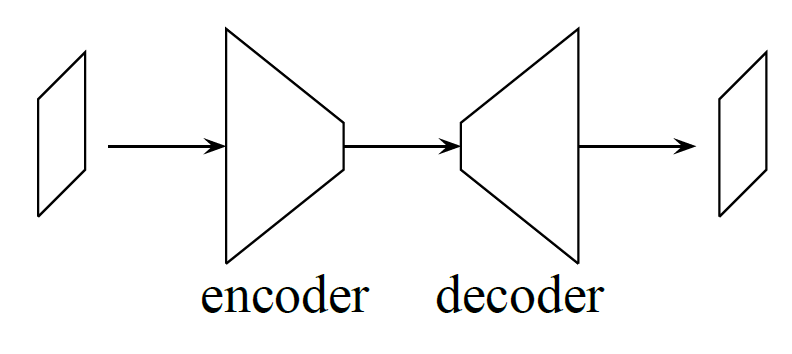
\includegraphics[width=0.6\linewidth]{Graphics/encoder-decoder.png}\\
    \end{multicols*}

    \subsection{Recurrent Neural Networks (RNN)}
    NN with feedback - nonlinear extension of IIR filters. (recursive)\\
    $\rightarrow$ memory of neurons: \textbf{sequential input-data} (temporal correlation)\\
    Training: SGD with $\utheta^{t+1} = \utheta^t - \gamma^t \nabla L(t, \utheta) |_{\theta = \theta^t}$
    (Difficult to train, vanishing gradients, hard to parallelize $\rightarrow$ sequential calculations)\\
    $\underline{s}_l(n) = \uphi_l \left( W_{l,x}\x_{l-1}(n) + W_{l,s}\underline{s}_{l}(n-1) + \underline{b}_l \right) $\\
    \subsubsection{Bidirectional recurrent neural networks (BRNN)}
    minibatch in forward- and backward-time direction in two separate recurrent layers; concatenate outputs ($\rightarrow$ next layer has past + future info)

    \subsubsection{Long short-term memory (LSTM)}
    Most successful type of RNN\\
    Replace recurrent neuron with \textbf{LSTM-cell(/neuron)}\\
     $\underline{s}_l(n) = \underline{f}_l(n) \odot \underline{s}_l(n-1) + \underline{i}_l(n) \odot \uphi _l\left( W_{l,sx}\x_{l-1}(n) + W_{l,so}\x_{l}(n-1) + \underline{b}_l \right) $ $\rightarrow$ no vanishing gradient in long memory\\
     \textbf{Peephole-LSTM:} gates depend on prev. state $\underline{s}_l(n-1)$\\
     more complex (11 weight matrices)\\
     \textbf{Gated recurrent unit (GRU):} lower complexity\\
     simplified: 2 gates (reset, update)\\

     \subsection{Transformer}
     multi-head self-attention; general purpose
     \begin{itemize}
         \item parallel computing (no recurrence)
         \item short- and long-range dependencies
         \item very high computation complexity (quadratic  $\mathcal{N}^2$)
         \item very high memory complexity
         \item requires more training data
     \end{itemize}
     \textbf{Tokenization:} divide text into known units (tokens) - by NN (e.g. \textit{Word2Vec})\\
     Positional encoding required for consideration of sequential order\\
     Feedforward dense layer: relationships within sequence\\

     \textbf{For images:} tokens for patches based on flattened 2D image-slices  


    \columnbreak


     \section{Self-supervised learning}
    To solve data-inefficiency of NN\\
    Self-supervised learning is representation-oriented
    \textbf{Self-supervised representation learning (SSL)}
    unlabeled dataset; mostly for pretraining\\
    \textbf{Semi-supervised learning}
    with small dataset; reduce labeling effort

    Split training in \textbf{pretraining}: model trained on other (more general?) dataset. Better than random params!\\
    Later \textbf{finetuning} with small labeled dataset (for downstream task) of whole model, or only head (with others params frozen)\\

    \textbf{Foundation models (FM)} are general-purpose models, trained on task-agnostic data
    
    \subsection{Autoencoder (AE)}
    encoder-decoder architecture; simplest SSL; undercomplete (inner dimension  $c \ll d$ input/output)\\
    input $\rightarrow$ encoder $\rightarrow$ latent variable $z$ (hidden, compressed representation) $\rightarrow$ decoder $\rightarrow$ loss against input $\y=\x$
    
    \subsection{Pretext task (PT)}
    Artificially generated supervised task\\
    self-reconstruction (autoencoder) $\in$ pretext task\\

    example-tasks: image rotation, colorization, masking, super-resolution.
    
    \subsection{Contrastive learning}
    learn contrast between similar/dissimilar samples\\
    \textbf{samples are generated}: 
    crop, resize, rotate, flip, color distortion, cutout, gaussian noise/blur, other filters, ...\\ 
    $\rightarrow$ No task, no $\y$, no supervised loss (loss in representation space)\\
    Goal for representation space $\underline{z}$:\\
    similar/dissimilar samples (positives/negatives) pulled/pushes to/from each other \\
    
    
    \section{Transfer learning}
    embedded systems: one model for one task (due to system-restraints)\\
    With \textbf{source task} $\mathcal{T}_s = \{ X_s, Y_s, p_s(\x,\y) \}$ \\
    Transfer learning applicable to \textbf{Related tasks} ($X_s=X_t,Y_s\neq Y_t$) and \textbf{Distribution/Domain shift} ($X_s=X_t, Y_s=Y_t, p_s(\x,\y) \neq p_t(\x,\y)$ - like cross sensor, cross daytime, ...)\\
    New task ($X_s\neq X_t$) is too difficult!

    \textbf{Related tasks:} Freeze backbone and train new head - or - multitask-training\\
    \textbf{Distribution/Domain shift:}\\
    - Domain adaptation (Transform new task to source-domain)\\
    - Continual learning (model must perform well in all new tasks), no catastrophical forgetting!
    
    
    \vfill\null    % ugly fix to achieve formatting
    \columnbreak

    \section{Generative models}
    learn joint distribution $p(\x,\y)$ (instead of focusing on decision boundaries like discriminative models) to generate new data according to $p(\x,\y)$

    \subsection{Variational autoencoder (VAE)}
    = AE with requirement: $z$ need to be known distribution\\
    $\rightarrow$ after training: draw sample from $z$, use decoder to generate output 

    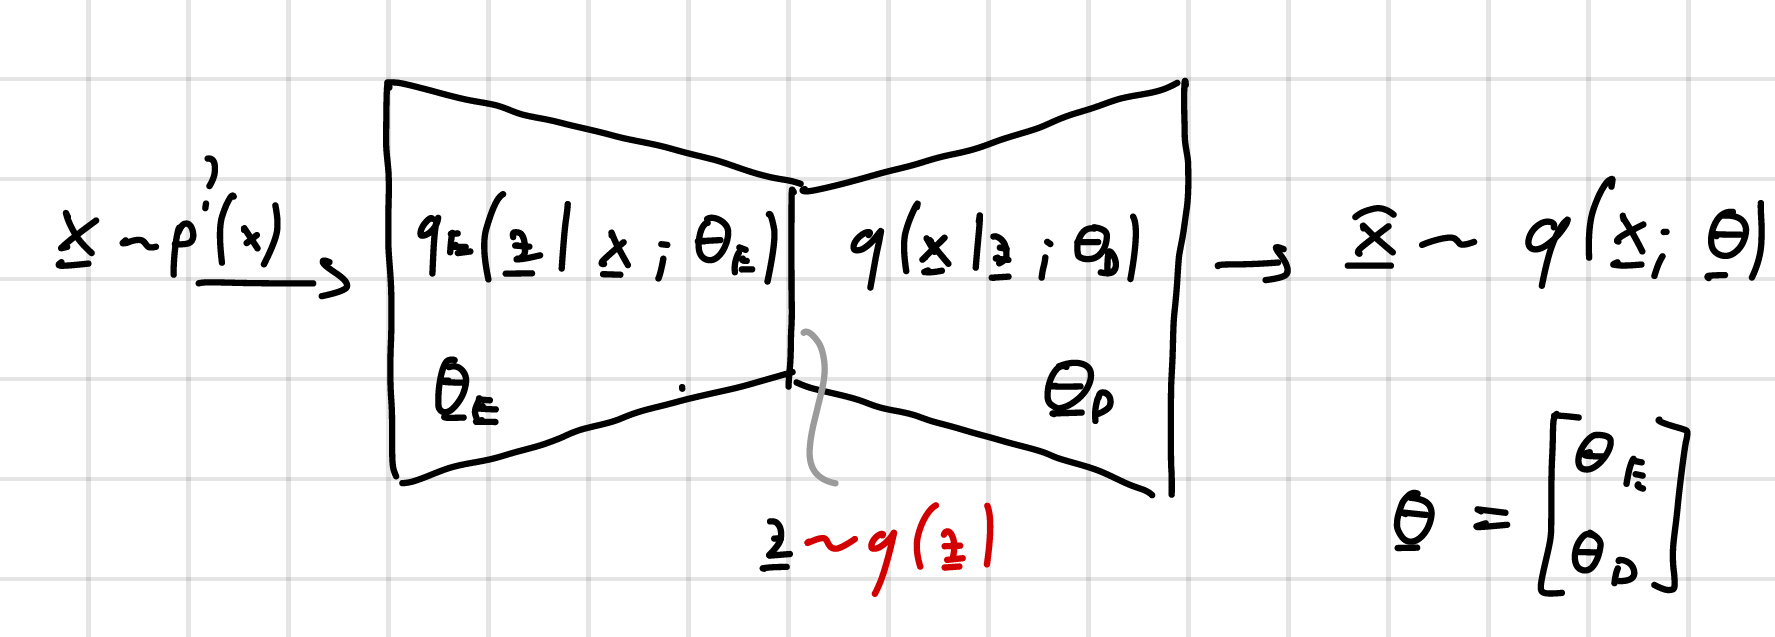
\includegraphics[width=0.6\linewidth]{Graphics/vae.png}\\
    $q(\x, \utheta)= \int q(\x, \underline{z}; \utheta ) d\underline{z} = \int q( \x \mid \underline{z}; \utheta) \cdot q(\underline{z}) d \underline{z}$
    for solution: replace $-\ln q(\x; \utheta)$ by its variational upper bound;
    use stochastic encoding + reparametrization (to enable backpropagation of gradient through sampling unit)\\
    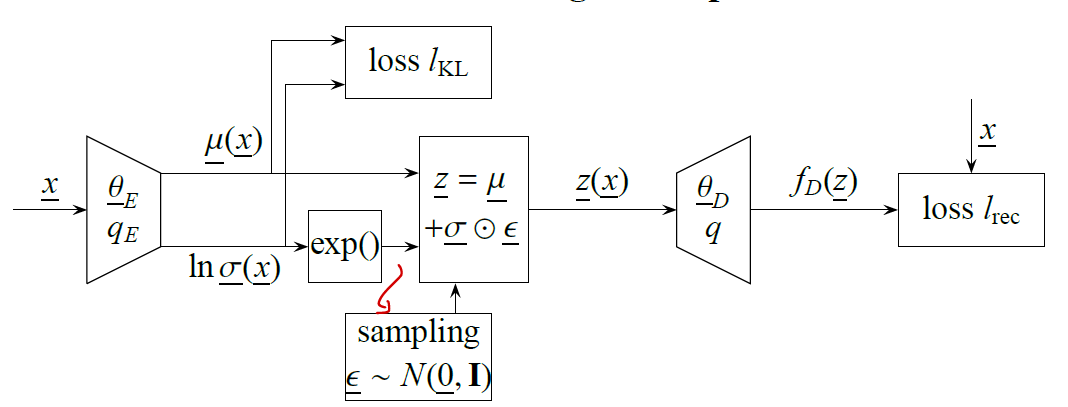
\includegraphics[width=0.8\linewidth]{Graphics/vae-stochasticEncoding-reparametrization.png}\\

    \subsection{Generative adversarial network (GAN)}
    More powerful than VAE;\\
    generator (G) vs discriminator (D), while generator has packpropagation from discriminator.\\
    min-max optimization: $\min_{\utheta_G}\max_{\utheta_D} L(\utheta_G, \utheta_D)$\\
    with $L(\utheta_G, \utheta_D) = \mathbb{E}_{\x\sim p_{\textrm{data}}} \ln(D(\x; \utheta_D)) + \mathbb{E}_{\underline{z}\sim p_{\textrm{noise}}} \ln\left(1 - D(G(\underline{z};\utheta_G); \utheta_D)\right)$

    Ping-Pong training:\\
    - one minibatch updating D ($\max_{\utheta_D} L(\ldots)$) 
        $\rightarrow$ stoch grad ascent \\
    - one minibatch updating G ($\min_{\utheta_G} L(\ldots)$) 
        $\rightarrow$ stoch grad descent\\
     $\rightarrow$ Nash-equilibrium (saddle point)\\
     difficult; mode collapse possible

     Generate realistic (fake) samples:
     data augmentation for training;
     data generation without privacy concerns.\\
     No control over output (from noise $\underline{z}$) - no labels used
     
     $\rightarrow$ Extension: \textbf{conditional GAN (cGAN):}\\
     + class label input $\y \sim p_\textrm{label}$ \\
     D accepts only if real AND matches label
     
     $\rightarrow$ Extension: \textbf{Paired image translation:}\\
     On paired data $(\x,\y)$ (e.g. semantic segmentation, day-night)

    \subsection{Diffusion model}
    high quality; simpler training than GAN; high complexity; long training
    \textbf{Forward process (diffusion process):}\\
    Input $\x_0$ to Gaussian noise $\mathcal{N}(0, I)$ by sequence of first-order Markov processes

   \textbf{Reverse process (generation process):}\\
   random sample  $\x_T \sim \mathcal{N}(0, I)$ backwards through Markov process
    


    \vfill\null    % ugly fix to achieve formatting
    \columnbreak
    

    \section{Gradient Descent}
    local search! \hspace{6pt} $-\underline{\nabla} f(\x)$ orthogonal to contour line (towards descent)
    $\gamma$: step-size / learning rate \\
    $\utheta^{t+1} = \utheta^t - \gamma^t \nabla L(\utheta)|_{\utheta=\utheta^t} $ \\
    No need to calc Hessian $\rightarrow$ much simpler
    \subsection{Stochastic Gradient Descent (SGD)}
    Batch gradient descent - more noisy than $L(\utheta)$\\
    Use Minibatch of size $B<<D_{\textrm{train}}$\\
    $\utheta^{t+1} = \utheta^t - \gamma^t \nabla L(\textcolor{red}{t}; \utheta)|_{\utheta=\utheta^t} $ \\
    $\uparrow$ minibatch size $\Rightarrow$ $\uparrow$ less noise, convergence, parallel processing
    \subsection{... with Momentum}
    improvement to SGD: $\utheta^{t+1} = \utheta^t + \Delta \utheta^t$ \\
    $\utheta^{t+1} = \utheta^t - \gamma^t \nabla L(t; \utheta)|_{\utheta=\utheta^t} + \textcolor{red}{\beta \Delta \utheta^{t-1}} $ \\
    mit $\Delta \utheta^t = \beta \Delta \utheta^{t-1} \textcolor{blue}{- \gamma^t \nabla L(t; \utheta)|_{\utheta=\utheta^t}} \ $ \textcolor{blue}{regular SGD} \\
    $0\leq \beta \leq 1 \quad \beta=0 \rightarrow \textrm{SGD}$ \\
    reduce noise in stochastic gradient; reduce oscillation; \textbf{accelerate} ill-conditioned \textbf{convergence}
    \textbf{Nesterov Momentum} + look-ahead gradient (ch. 5.5)
    

    \subsection{Input normalization}
    \textbf{covariate shift:} change of distribution of input data over time.\\
    or large offset between channels.\\
    Input normalization over whole dataset (individually per channel) $x_i = \frac{x_i - \mu_i}{\sigma_i}$\\
    zero-mean unit-variance normalization decouples layers $\rightarrow$ easier  training\\
    \textbf{Batch normalization:} fix internal covariance shift over layers and time\\
    input normalization for hidden layers and each minibatch
    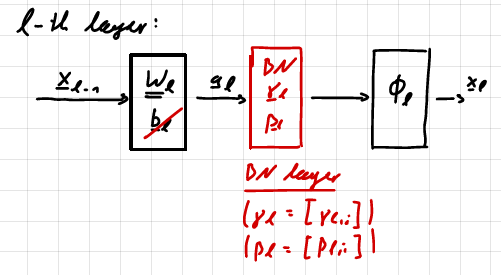
\includegraphics[width=0.4\linewidth]{Graphics/batch-normailzation.png}
    (During inference exponentially weighted averages of the training values are used)
    

    \subsection{Optimization Difficulties}
    \textbf{- stochastic gradient}\\
    \textbf{- ill conditioning}\\
    \begin{multicols*}{2}
         contour lines curvatures strongly different\\
        \columnbreak
        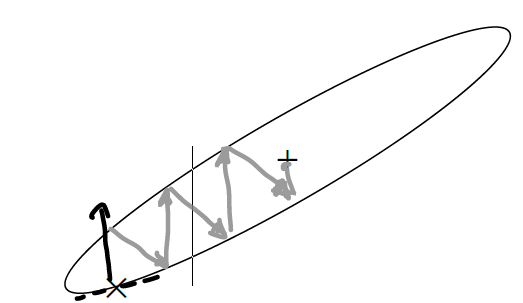
\includegraphics[width=0.5\linewidth]{Graphics/ill-conditioning.png}
    \end{multicols*}
    \textbf{- covariate shift}
    
    \textbf{- saddle point / plateau}\\
    verry slow convergence, as $\nabla L(\utheta) \approx 0$ - 
    some parameters have a very small influence\\
    \textbf{- sensitive to step size}\\
    slow convergence vs. oscillation (with overshoots) and no convergence\\
    $\Rightarrow$ learning rate decay:
    \begin{enumerate}
        \item Static schedule independent of $\utheta^t$:  (Step decay, Inverse time decay, Exponential decay)
        \item Adaptive schedules: \\
            RMSprop (root mean square propagation)\\
            Adam (adaptive moment estimation) \\
            AdaGrad (adaptive gradient algorithm)
    \end{enumerate}
    \textbf{- local minimum}\\
    \textbf{- vanishing gradient (or exploding)}\\
    Backpropagation of ''error vector'' $J_L(\underline{a}_L) = \frac{\partial L}{\partial \underline{a}_L}$ \\
    If $\forall L: ||J_{a_{l+1}}(a_l) || \gtrless 1 \ \rightarrow_{l\rightarrow 1} ||J_L(a_l) || = \begin{matrix} \infty \\ 0 \end{matrix} $ \\
    More serious for deep layers.\\
    ReLU less serious that e.g. Sigmoid 
    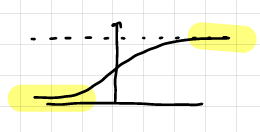
\includegraphics[width=0.25\linewidth]{Graphics/sigmoid.png}    

    other options:\\
    \begin{itemize}
        \item gradient clipping
        \item better optimization algorithm (adam)
         \item skip-connections in architecture
    \end{itemize}
    \hrule
    
    \section{Regularization}
    techniques to prevent overfitting
    \subsection{Model capacity}
    Ability of themodel to learn amapping\\
    too simple model $\rightarrow$ underfitting \\
    too complex model $\rightarrow$ overfitting \\

    \textbf{weight norm penalty}
    regularized cost function: $L_r(\theta) = L(\theta) + \sum_l \lambda_l P(W_l)$
    with penalty-term $P$ and regularization parameter $\lambda$

    (large weights tends to overfitting)
    
    \textbf{early stopping}\\
    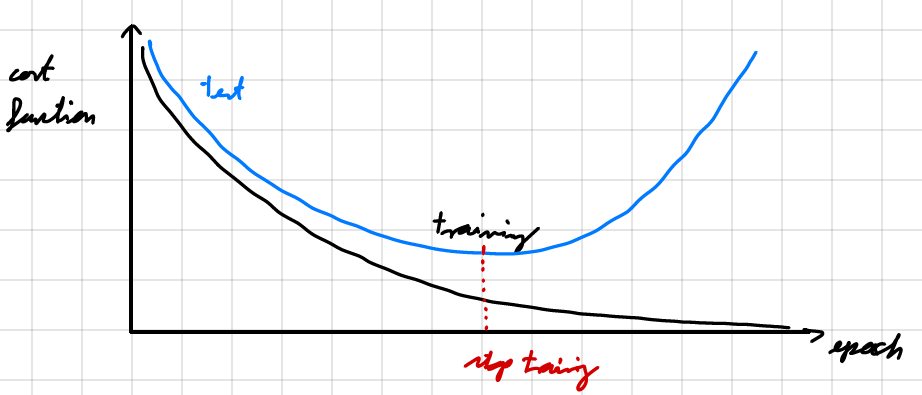
\includegraphics[width=0.7\linewidth]{Graphics/early-stopping.png}\\
    
    \textbf{data augmentation}
    use artificial but realistic training samples to increase training-material $\rightarrow$ better model\\
    modify data without changing class labels: 
    translation/rotation/scaling/flip, added noise, modified colors / textures, use of image patches, ...
    
    \textbf{ensemble learning}
    train different models (training data subsets, architecture, cost functions, optimizer, ...)\\
    combine models (regression: average; classification: voting)
    
    \textbf{dropout}
    (Implicit ensemble learning method) \\
    randomly removes neurons based on dropout rate $d_l$.
    outgoing weights corrected by $(1-d_l)$

    \subsection{Model reduction}
    Reduce computational/memory complexity and power consumption\\
    \textbf{Low-rank factorization:} $\tensr{W} \in \mathbb{R}^{M\times N} \approx \tensr{A}\tensr{B} \in \mathbb{R}^{M\times K} \cdot \mathbb{R}^{K\times N}$ reduces $MN$ to $(M + N)K$ multiplications\\
    \textbf{Pruning:} Force $\approx$ zero columns/rows in $\tensr{W}$, remove the corresponding neurons\\
    \textbf{Quantization:} reduce word length
    
\end{multicols*}
\end{document}
